%% Revised manuscript (Elsevier, elsarticle). Build: pdflatex main; bibtex main; pdflatex main; pdflatex main
%% Every number is generated by the scripts named in docs/results-corrected.md.
\documentclass[preprint,12pt]{elsarticle}
\usepackage[T1]{fontenc}
\usepackage{lmodern}
\usepackage{amsmath,amssymb}
\usepackage{graphicx}
\usepackage{booktabs}
\usepackage{multirow}
\usepackage{xcolor}
\usepackage{url}
\usepackage[hidelinks]{hyperref}
\graphicspath{{figures/}}
\newcommand{\pending}[1]{\textcolor{red}{[#1]}}

\journal{Pervasive and Mobile Computing}

\begin{document}

\begin{frontmatter}

\title{Can Ambient WiFi Support Vehicular Multipath SLAM? Virtual-Anchor Localization,
Commodity Front-End Limits, and a Delay-Convention Pitfall in Ray-Traced Evaluation}

\author{Mulham Fetna\corref{cor1}}
\ead{contact@mulhamfetna.com}
\cortext[cor1]{Corresponding author. ORCID: 0009-0006-4432-798X.}
\affiliation{organization={Department of Mechatronics Engineering, University of Aleppo},
            city={Aleppo},
            country={Syria}}

\begin{abstract}
Ambient WiFi is radiated by existing infrastructure and received by hardware a vehicle already
carries, which makes it an attractive low-cost aid for vehicular simultaneous localization and
mapping (SLAM). We ask what commodity channel state information (CSI) can actually contribute,
using ray-traced channels (Sionna RT) in three outdoor scenarios, wheel-grade odometry as the
baseline that any aid must beat, and a virtual-anchor FastSLAM back-end in which each wall
reflection is represented by the access point mirrored in that wall. With exact multipath
parameters the geometry works: WiFi reduces odometry drift by 66--79\,\% and, beside a single
reflecting wall, outperforms a simulated spinning LiDAR. With a commodity front-end it does not:
joint delay--angle MUSIC on a four-element linear array returns only about 15\,\% facade
reflections, about a third of detections match no propagation path, and a further 19--34\,\% are
real paths reported at their front/back mirror angle. These errors persist across frames, are
confirmed as false anchors, and make WiFi-aided SLAM worse than dead reckoning in every scenario;
the share of unexplained detections does not fall with bandwidth from 20 to 160\,MHz. We also
report a delay-convention pitfall in ray-traced CSI studies: channel frequency responses whose
delays are referenced to the first arrival, as on real hardware, were read as absolute path
lengths in our earlier analyses. This produced a spurious several-metre range bias and an
inflated phantom rate, both of which vanish once excess delay is modelled explicitly. Code,
cached channels, and firmware are released openly.
\end{abstract}

\begin{keyword}
WiFi sensing \sep channel state information \sep multipath-assisted SLAM \sep virtual anchors
\sep vehicular localization \sep ray tracing
\end{keyword}

\end{frontmatter}

%% ===========================================================================
\section{Introduction}\label{sec:intro}

Exteroceptive sensors are the expensive part of a vehicle's localization and mapping stack.
WiFi is the opposite: access points (APs) already illuminate most built environments, and
commodity receivers that report channel state information (CSI) cost a few dollars. Multipath
components in that CSI carry geometric information, since each specular reflection arrives
along a path whose length and angle are fixed by the reflector and the transmitter
\cite{leitinger2015jsac,gentner2016channelslam}. Whether a moving vehicle can turn that
information into better localization, or into a map, depends on two separate questions: is the
geometry informative, and can a commodity front-end extract it?

This paper separates those questions. We evaluate ambient-WiFi SLAM in ray-traced outdoor
scenes against the baseline that matters for a vehicle, wheel-grade odometry, and against a
simulated LiDAR given the same odometry. The back-end is a virtual-anchor FastSLAM
\cite{montemerlo2002fastslam}: each wall reflection is represented by the AP mirrored in that
wall, a point that is fixed in the world and whose range equals the bistatic path length. We
feed it either exact multipath parameters (an oracle) or the output of joint delay--angle MUSIC
\cite{schmidt1986music,shan1985smoothing} applied to noisy CSI from a four-element array.

The work also corrects our own earlier analyses \cite{fetna2026wifiradar}, which reported
centimetre-level WiFi localization at parity with LiDAR and attributed a mapping failure to a
``phantom ceiling'' with a several-metre range bias. Re-verification found three defects: the
estimator was driven by ground-truth odometry, its measurement update carried no position
information, and CSI delays referenced to the first arrival were read as absolute path lengths.
Section~\ref{sec:pitfall} documents the last of these, because it is easy to repeat in any
study that synthesizes CSI from a ray tracer.

\paragraph{Contributions}
\begin{itemize}
  \item A ray-traced evaluation of ambient-WiFi vehicular SLAM with a realistic odometry
        baseline, paired LiDAR runs, a straight and a lane-change trajectory, and ten seeds
        (Sections~\ref{sec:method}--\ref{sec:results}).
  \item Evidence that the virtual-anchor geometry is informative: exact multipath parameters
        reduce odometry drift by 66--79\,\% (Section~\ref{sec:loc}).
  \item A decomposition of what a commodity front-end returns, showing that unexplained
        detections and single-array front/back folding, not range resolution, prevent that
        gain from being realized (Sections~\ref{sec:frontend}--\ref{sec:bw}).
  \item A description of the excess-delay pitfall, its quantitative effect, and a measurement
        model that handles it (Section~\ref{sec:pitfall}).
  \item Hardware evidence from two ESP32-S3 boards that commodity CSI indeed fixes delays only
        relative to the first arrival (Section~\ref{sec:hw}), and an open artifact.
\end{itemize}

%% ===========================================================================
\section{Related work}\label{sec:related}

\textbf{WiFi and CSI sensing} is mature for indoor, largely static settings: through-wall and
device-free sensing \cite{chetty2012ttwifi,zhao2018rfpose,zhao2018rfpose3d}, CSI ranging and
imaging \cite{li2021standalone,wang2025csipower,maatta2024csipointcloud}, and pose recovery
\cite{geng2022denseposewifi,yan2024personinwifi3d}. Decimetre AP-side localization with
super-resolution has been shown with commodity cards \cite{kotaru2015spotfi}, and the lack of
absolute time of flight in commodity CSI is well documented \cite{xie2015pdp}; it is the reason
the delay convention in Section~\ref{sec:pitfall} matters.

\textbf{Multipath-assisted localization and SLAM} treats specular reflections as virtual
anchors whose positions are learned jointly with the agent's
\cite{leitinger2015jsac,gentner2016channelslam,ulmschneider2017multipath,leitinger2024mpslamcoop,li2024bpmpslam}.
These systems typically use wideband, synchronized, or carefully calibrated signals. WiFi-based
SLAM otherwise localizes against known APs or radio fingerprints
\cite{arun2022p2slam,liu2023radiofingerprintslam}, or uses WiFi to assist a primary sensor
\cite{arun2022viwid,ismail2022wifilidarslam,li2025ekfwifilidarimu}.

\textbf{Integrated sensing and communication} envisions shared waveforms for both functions
\cite{liu2022isac,zhang2021jcassurvey,xiong2023scfundamental,overview2024ieee80211bf}; 60\,GHz
802.11ad has been used as a radar \cite{kumari2018adradar,han2022adimaging}, and a passive radar
on a moving platform has been demonstrated with 5G \cite{maksymiuk2024movingpr}. Our setting,
ambient sub-7\,GHz WiFi received on a moving vehicle outdoors with commodity array sizes, sits
between these lines; the question we answer is how much of the multipath-SLAM machinery survives
a commodity front-end.

%% ===========================================================================
\section{System model and method}\label{sec:method}

\subsection{Bistatic geometry and virtual anchors}
A vehicle at horizontal position $\mathbf{p}$ receives signals from $N_\mathrm{AP}$ ambient APs at
known positions $\mathbf{a}_i$. A single specular reflection from a planar facade follows the
path $\mathbf{a}_i\rightarrow\mathbf{r}\rightarrow\mathbf{p}$; mirroring the AP in the facade
gives the virtual anchor (VA) $\mathbf{v}$, and the reflection is indistinguishable from a
line-of-sight (LOS) signal from $\mathbf{v}$:
\begin{equation}
\rho = \lVert\mathbf{v}-\mathbf{p}\rVert,\qquad \phi = \operatorname{atan2}(\mathbf{v}-\mathbf{p}),
\label{eq:va}
\end{equation}
where $\rho$ is the (horizontal) bistatic path length and $\phi$ the arrival azimuth. Because
$\mathbf{v}$ is fixed in the world, repeated observations constrain $\mathbf{p}$. The reflection
point $\mathbf{r}$ follows from $(\rho,\phi)$ and $\mathbf{a}_i$ by the bistatic ellipse solve and
is what we map. All lengths are projected to the ground plane using the known AP and receiver
heights, which a facade bounce preserves.

\subsection{Excess-delay measurement model}
Commodity CSI does not provide absolute time of flight; delays are known only relative to the
first arrival \cite{xie2015pdp}. With an LOS first arrival the measured excess length is
\begin{equation}
e = \rho_\mathrm{3D} - \lVert\mathbf{a}_i - \mathbf{p}\rVert_\mathrm{3D}
\quad\Longrightarrow\quad
\rho_\mathrm{3D}(\mathbf{p}) = e + \lVert\mathbf{a}_i - \mathbf{p}\rVert_\mathrm{3D},
\label{eq:excess}
\end{equation}
so the path length used in \eqref{eq:va} depends on the hypothesized pose and the AP position.
The filter evaluates \eqref{eq:excess} per particle. This is the model whose omission is
discussed in Section~\ref{sec:pitfall}.

\subsection{Odometry}
Wheel odometry is modelled with a per-run scale error ($\sigma=1\,\%$), an initial heading error
($\sigma=0.5^\circ$), a heading random walk ($0.2^\circ/\sqrt{\mathrm{s}}$), and white velocity
noise ($0.05$\,m/s). Dead reckoning on this odometry is reported beside every result, and the
WiFi and LiDAR runs of a given seed use the identical odometry draw.

\subsection{Virtual-anchor FastSLAM}
Each of 200 particles carries a pose and an extended Kalman filter per VA
\cite{montemerlo2002fastslam}. A detection is associated, per particle, with the VA of the same AP
that minimizes the Mahalanobis distance of $(\rho,\phi)$, gated at the 99\,\% $\chi^2_2$ level;
associated detections update the VA and weight the particle by the innovation likelihood, and
unexplained detections initialize a tentative VA. A VA is confirmed after five associations, and
a tentative VA unseen for ten frames is deleted. The map consists of reflection points of
detections associated with confirmed VAs, located from the posterior pose. Measurement standard
deviations are fixed a priori: $0.3$\,m and $2^\circ$ for the oracle, $0.5\,c/B$ and $5^\circ$ for
MUSIC at bandwidth $B$. A single uniform linear array (ULA) reports only the forward azimuth
branch; an optional \emph{two-branch} model scores each detection against both $\phi$ and
$\pi-\phi$ and seeds a tentative VA for each.

\subsection{Channels, scenes, and front-ends}
Channels are ray traced with Sionna RT 2.0 \cite{hoydis2023sionnart} at 5.2\,GHz (maximum depth
three) and stored once per scene, including the noise-free channel frequency response at 20, 40,
80, and 160\,MHz and the full table of propagation paths. Seeds vary the receiver noise (20\,dB
SNR) and the odometry. The receiver is a four-element half-wavelength ULA with 128 subcarriers.
Three scenarios are used: a \emph{controlled} metal wall (30\,m, 120 frames, three APs), a
\emph{street canyon} with metal facades (60\,m, 240 frames, three APs), and the same canyon driven
on a lane-change S-curve of 2.5\,m amplitude. The \emph{oracle} front-end uses the true
single-scatter, non-floor paths in the excess-delay convention; the \emph{realistic} front-end is
joint 2-D MUSIC with 2-D spatial smoothing \cite{schmidt1986music,shan1985smoothing} estimating
three paths per AP.

\subsection{Baseline and metrics}
The LiDAR baseline is an Ouster-class scanner ray-cast against the scene geometry with a
scan-to-map ICP back-end, externally validated on KITTI sequence 04 (1.16\,m absolute trajectory
error over 394\,m) \cite{geiger2012kitti}, and seeded with the same noisy odometry. We report the
absolute trajectory error (ATE), occupancy intersection-over-union (IoU, 1\,m cells) against
facade footprints, and map accuracy. To characterize the front-end, every detection is matched
per frame to the true paths of the same AP using the normalized cost
$\sqrt{(\Delta\rho/3\,\mathrm{m})^2+(\Delta\phi/10^\circ)^2}\le3$; a detection that matches only
after mirroring the true azimuth onto the forward branch is counted as \emph{folded}, and one
that matches neither is \emph{unexplained}.

%% ===========================================================================
\section{Results}\label{sec:results}

Results are mean $\pm$ standard deviation over ten seeds at 160\,MHz unless stated otherwise.

\subsection{Localization}\label{sec:loc}

\begin{table}[t]\centering\small
\caption{Absolute trajectory error (m) under wheel-grade odometry, ten seeds.}
\label{tab:ate}
\begin{tabular}{@{}lccc@{}}
\toprule
 & Controlled wall & Street canyon & Street, S-curve \\ \midrule
Dead reckoning              & $0.211\pm0.109$ & $0.470\pm0.260$ & $0.472\pm0.259$ \\
WiFi, oracle                & $\mathbf{0.072\pm0.026}$ & $0.101\pm0.045$ & $0.100\pm0.047$ \\
WiFi, MUSIC                 & $0.340\pm0.123$ & $1.202\pm0.241$ & $1.065\pm0.199$ \\
WiFi, MUSIC, two-branch     & $0.390\pm0.110$ & $0.527\pm0.167$ & $0.488\pm0.266$ \\
LiDAR (ICP)                 & $0.172\pm0.117$ & $\mathbf{0.027\pm0.001}$ & $\mathbf{0.028\pm0.000}$ \\
\bottomrule
\end{tabular}
\end{table}

\begin{figure}[t]\centering
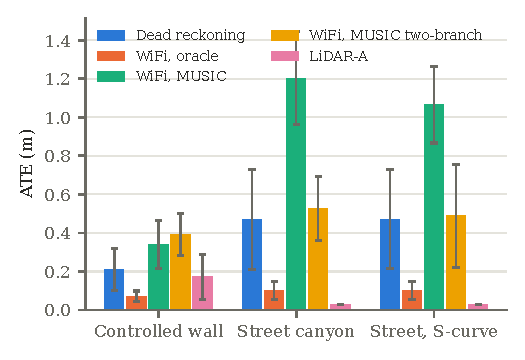
\includegraphics[width=0.75\linewidth]{localization.pdf}
\caption{Trajectory error under the same wheel-grade odometry. Exact multipath parameters make
WiFi a useful aid; joint MUSIC on a four-element array makes it harmful.}
\label{fig:loc}
\end{figure}

Table~\ref{tab:ate} and Fig.~\ref{fig:loc} give the central result. With exact multipath
parameters, WiFi reduces the odometry error by 66\,\% beside the single wall and by 79\,\% in both
street runs; the filter confirms exactly the three and seven VAs present. Beside a single wall
WiFi also outperforms LiDAR, whose scan matching cannot constrain motion along a featureless
plane, whereas the VAs of three APs observe the wall from different directions. In the street
canyon LiDAR is four times better again.

With the realistic front-end the same filter is worse than dead reckoning in every scenario.
It confirms 28 VAs beside the wall and 101--116 in the canyon, against three and seven real ones:
erroneous detections recur from frame to frame often enough to pass the five-observation
promotion test, and once confirmed they pull the particles. The two-branch model, which accounts
for the array's front/back ambiguity, removes most of the excess error in the canyon but only
reaches dead-reckoning parity. The trajectory shape makes no material difference.

\subsection{What the commodity front-end returns}\label{sec:frontend}

\begin{figure}[t]\centering
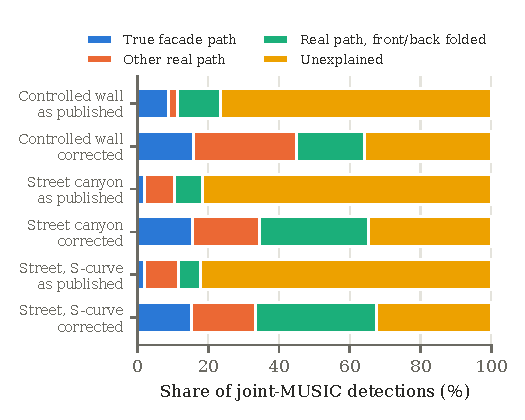
\includegraphics[width=0.75\linewidth]{frontend_decomposition.pdf}
\caption{Composition of joint-MUSIC detections, as published in our earlier analysis (excess
delay read as absolute length) and corrected. Only about 15\,\% of detections are facade
reflections in every scenario.}
\label{fig:frontend}
\end{figure}

\begin{table}[t]\centering\small
\caption{Composition of joint-MUSIC detections (\%) and median signed range error of matched
facade detections, at 160\,MHz.}
\label{tab:frontend}
\begin{tabular}{@{}lccc@{}}
\toprule
 & Controlled & Street & S-curve \\ \midrule
True facade path              & 15.7 & 15.5 & 15.2 \\
Other real path (LOS, floor, multi-bounce) & 29.2 & 19.0 & 18.2 \\
Real path, front/back folded  & 19.3 & 30.8 & 34.1 \\
Unexplained                   & 35.8 & 34.6 & 32.4 \\ \midrule
Facade range error, corrected (m) & $+0.03$ & $-0.06$ & $-0.06$ \\
\emph{As published:} unmatched share & 88.8 & 89.7 & 88.5 \\
\emph{As published:} facade range error (m) & $-6.35$ & $-2.19$ & $-6.62$ \\
\bottomrule
\end{tabular}
\end{table}

Table~\ref{tab:frontend} and Fig.~\ref{fig:frontend} explain the localization failure. Only one
detection in six is a facade reflection, the only kind that defines a VA. A fifth to a third are
genuine paths reported at their mirror angle, which a single ULA cannot resolve; these are not
estimator artefacts, and a second array axis or a vehicle-heading change would disambiguate them.
About a third match no propagation path within the generous tolerance. The facade detections
that are found are accurate in range (median error below 0.1\,m), so the problem is not bias or
precision but the composition of the detection set.

\subsection{Mapping under ground-truth poses}\label{sec:map}

\begin{figure}[t]\centering
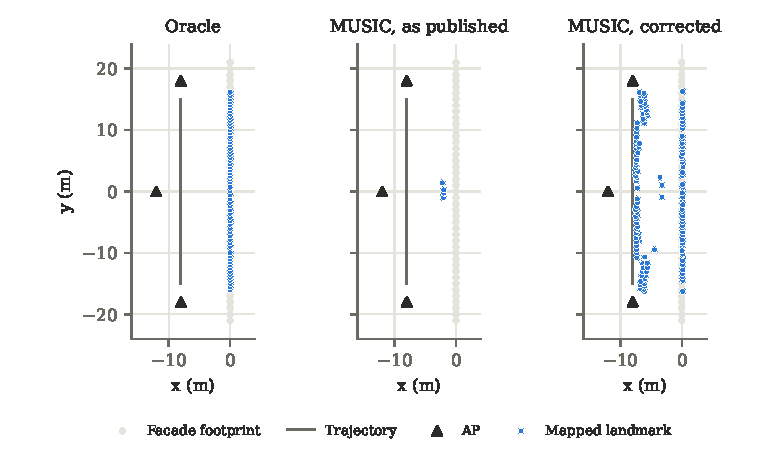
\includegraphics[width=0.85\linewidth]{maps_controlled.pdf}
\caption{Maps of the controlled wall triangulated at ground-truth poses (one seed). The
as-published reading of the realistic detections places almost nothing on the wall; with the
excess-delay model the wall is recovered, together with clutter near the trajectory.}
\label{fig:maps}
\end{figure}

Scoring the map at ground-truth poses isolates the front-end from localization. Beside the wall
the oracle reaches an IoU of 0.767 and MUSIC 0.349\,$\pm$\,0.017 (Fig.~\ref{fig:maps}); the
as-published reading scored 0.000. In the canyon the oracle itself reaches only 0.075, because
three APs illuminate a small fraction of the facade footprints, and MUSIC reaches 0.03. Mapping of
the illuminated facades is therefore possible with commodity CSI in a clean geometry, but it
carries clutter from the misplaced detections and is bounded by illumination coverage.

\subsection{Bandwidth}\label{sec:bw}

\begin{table}[t]\centering\small
\caption{Joint-MUSIC detection composition and ground-truth-pose map IoU versus bandwidth
(five seeds).}
\label{tab:bw}
\begin{tabular}{@{}lcccc@{}}
\toprule
 & \multicolumn{2}{c}{Controlled} & \multicolumn{2}{c}{Street} \\
Bandwidth & Unexplained (\%) & IoU & Unexplained (\%) & IoU \\ \midrule
20\,MHz  & 44.4 & 0.474 & 37.7 & 0.012 \\
40\,MHz  & 36.9 & 0.341 & 43.3 & 0.020 \\
80\,MHz  & 35.9 & 0.331 & 33.3 & 0.027 \\
160\,MHz & 35.8 & 0.349 & 34.6 & 0.031 \\
\bottomrule
\end{tabular}
\end{table}

Eightfold more bandwidth does not reduce the unexplained share (Table~\ref{tab:bw}). The limit is
set by the four-element aperture and by model mismatch in a coherent, single-snapshot multipath
channel, not by range resolution.

\subsection{Robustness to AP-position error and measurement loss}\label{sec:robust}

Unlike in our earlier analysis, AP-position error now enters the measurement through
\eqref{eq:excess}, and measurement loss now matters because the odometry drifts.
Fig.~\ref{fig:robust} reports five seeds per point; dead reckoning is 0.158\,m (controlled) and
0.370\,m (street) for these seeds. \textbf{AP-position error is critical.} With exact multipath
parameters the oracle's advantage over odometry disappears once the AP coordinates are wrong by
about 0.5\,m beside the wall (0.242\,m against 0.158\,m) and by about 1\,m in the canyon
(0.479\,m against 0.370\,m); at 8\,m of error the oracle is two to three times worse than dead
reckoning. Every excess-delay measurement inherits the AP error through \eqref{eq:excess}, so an
ambient-WiFi aid requires AP positions surveyed to sub-metre accuracy, or estimated jointly.
\textbf{Measurement loss is tolerated.} A total blackout of 40 frames (17\,\% of the street run,
33\,\% beside the wall) raises the oracle's error only from 0.083 to 0.106\,m in the canyon and from
0.057 to 0.074\,m beside the wall; the filter falls back on odometry and re-acquires the confirmed
VAs. For MUSIC, removing measurements makes the error \emph{smaller} (1.277 to 0.796\,m for an
80-frame blackout in the canyon), consistent with its detections doing harm.

\begin{figure}[t]\centering
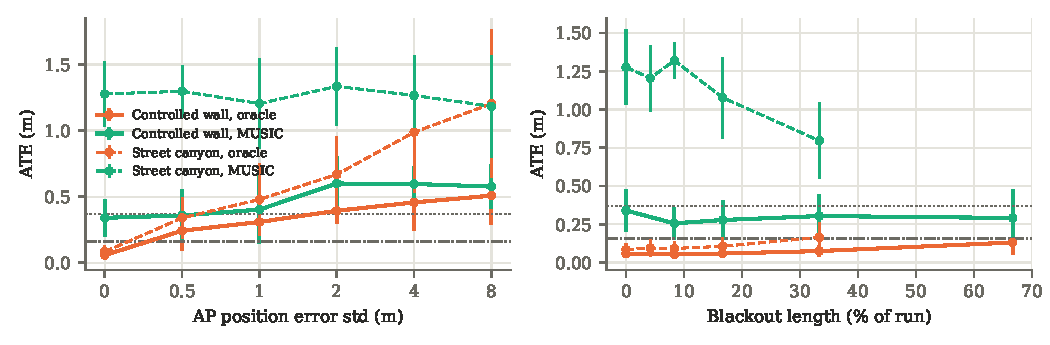
\includegraphics[width=\linewidth]{robustness.pdf}
\caption{Sensitivity to AP-position error (left) and to a total measurement blackout starting at
one third of the run (right); solid: controlled wall, dashed: street canyon; horizontal lines:
dead reckoning. Five seeds.}
\label{fig:robust}
\end{figure}

\subsection{Geometry, carrier, and bandwidth: the radar ablation}\label{sec:ablation}

\pending{Re-run of the CFAR ablation (cells A--D) and of the MUSIC row with the excess-delay
correction (M$^\ast$) from results/ablation\_*.json.}

%% ===========================================================================
\section{The excess-delay pitfall}\label{sec:pitfall}

Sionna RT's channel-frequency-response routine references all delays to the first arriving
path by default. That is realistic, because commodity CSI has no absolute time of flight, but a
back-end that treats the resulting delays as absolute bistatic path lengths under-ranges every
detection by the LOS distance $\lVert\mathbf{a}_i-\mathbf{p}\rVert$. In our earlier analyses this
produced three findings that were artefacts: a median range bias of several metres (6.35\,m beside
the wall; 0.03\,m once corrected), an unmatched share near 89\,\% (55--67\,\% corrected, of which a
third to a half is front/back folding), and a map IoU of zero at ground-truth poses (0.349 beside
the wall corrected). It also explains why the earlier mapping floor did not move with bandwidth or
aperture: no resolution can remove an offset equal to the LOS distance. The radar chain in the
same code read absolute delays directly and was unaffected.

Two safeguards would have caught it. First, triangulating the \emph{true} path parameters and the
\emph{estimated} ones at ground-truth poses and comparing the two isolates any systematic offset
in the estimator chain. Second, a synthetic single-path test of the full chain, from CSI
synthesis through detection, exposes a reference-convention mismatch immediately. We recommend
both for any study that synthesizes CSI from a ray tracer.

%% ===========================================================================
\section{Hardware: what commodity CSI provides}\label{sec:hw}

Two ESP32-S3 boards \cite{espressif_esp32,hernandez2020esp32}, one transmitting HT40 frames and one
logging CSI, were used to confirm the measurement convention on real silicon. From a static
capture we parse valid 40\,MHz high-throughput records whose long training field carries 128
subcarriers with 114 non-null, matching the physical active mask. The delay profile obtained by
coherent averaging places the LOS tap at zero delay with no absolute reference, which is the
excess-delay convention of \eqref{eq:excess}. This bench validates the CSI reading and the
convention, not a SLAM system; measuring detection composition against surveyed reflectors on
this hardware requires a large surveyed space and is left as future work. The firmware and the
offline chain are released so that the measurement can be reproduced for the cost of two
development boards.

%% ===========================================================================
\section{Discussion}\label{sec:discussion}

\textbf{What would close the gap.} The oracle results show that the geometry is informative
enough to matter. The realistic results identify what stands in the way, in order of share: an
unexplained third of the detections, front/back folding, and non-facade real paths. Folding is a
property of the single linear array and would be removed by a second array axis or by exploiting
heading changes; the unexplained detections call for front-ends with explicit model-order
selection or sparse estimation, and for VA promotion rules that test geometric consistency rather
than mere persistence.

\textbf{Limitations.} All channels are simulated; the hardware result confirms the measurement
convention, not the detection statistics. The scenes use perfectly conducting facades, which
favour specular reflection. Three APs is a modest density, which limits map coverage in the
canyon. The LOS-first assumption in \eqref{eq:excess} fails where the direct path is blocked.
Heading is assumed known for converting array angles to world azimuth.

\textbf{Correction of earlier claims.} Our earlier unpublished manuscripts reported WiFi
localization at parity with LiDAR, robustness to AP-position error and to measurement blackouts,
a fusion design rule, and cost-normalized accuracy. Those results relied on ground-truth odometry
and a measurement update without position information and are withdrawn; the mapping-mechanism
results that relied on the delay convention are corrected in Section~\ref{sec:pitfall}.

%% ===========================================================================
\section{Conclusion}\label{sec:conclusion}

Ambient WiFi received on a vehicle carries enough multipath geometry to reduce wheel-odometry
drift substantially when reflections are estimated exactly, and a virtual-anchor FastSLAM uses it
without knowing the facades in advance. A commodity four-element array with joint MUSIC does not
deliver that geometry: most detections are not facade reflections, a large share are mirrored by
the array's front/back ambiguity, and the errors persist long enough to be confirmed as anchors,
so WiFi-aided SLAM ends up worse than odometry alone. Bandwidth does not change this. Mapping of
illuminated facades is possible at known poses. Finally, ray-traced CSI studies must model delays
relative to the first arrival explicitly; reading them as absolute path lengths manufactures a
range bias and a phantom rate that are not properties of the sensor.

\section*{Data and code availability}
All code, configurations, cached ray-traced channels (regenerable), result files, and ESP32
firmware are available under AGPL-3.0 at \url{https://github.com/mulhamfetna/wifi-radar-slam}.

\section*{Declaration of competing interest}
The author declares no competing interests.

\section*{Funding}
This research did not receive any specific grant from funding agencies in the public,
commercial, or not-for-profit sectors.

\bibliographystyle{elsarticle-num}
\bibliography{refs}

\end{document}
